\documentclass[pra,aps,twocolumn,nofootinbib,superscriptaddress]{revtex4-2}

\usepackage{amsmath,amssymb,mathtools}
\usepackage{bm}
\usepackage{graphicx}
\usepackage{microtype}
\usepackage[hidelinks]{hyperref}

\newcommand{\Tr}{\operatorname{Tr}}
\newcommand{\W}{\mathcal{W}}
\newcommand{\Dset}{\mathcal{D}}

\begin{document}

\title{Two-use additivity of output ergotropy for generalized amplitude damping}

\author{Xiaojian Zeng}
\email{xiaojianzeng@foxmail.com}
\affiliation{PBC School of Finance, Tsinghua University, Beijing 100190, China}

\date{\today}

\begin{abstract}
We consider two noninteracting unit-gap qubits subjected independently to the
same generalized amplitude-damping channel.  At a fixed upper bound on the
mean input energy, we optimize the output ergotropy over all complex density
operators and allow a global work-extraction unitary.  A previous numerical
study found no two-use advantage and conjectured additivity, but its reduction
to real amplitudes does not cover the full input set.  We prove exactly that
the unrestricted two-use optimum equals twice the one-use optimum for every
damping parameter $\gamma\in[0,1]$, equilibrium excitation
$\eta\in[0,1/2]$, and per-cell budget $e\in[0,1]$.  The proof first reduces
the energy-ball optimization to pure inputs while retaining the one invariant
two-qubit phase.  It then converts ergotropy to an output spectral-diameter
bound.  Exact formulas for the second and fourth elementary spectral
coefficients reduce the problem to a quadratic inequality, which is closed by
a sign-definite multiplier identity.  Thus entangling two-cell encodings
cannot increase maximal extractable work in this model.  The result concerns
exactly two parallel uses and does not establish additivity for arbitrary
numbers of cells.
\end{abstract}

\maketitle

\section{Introduction}

Ergotropy quantifies the work extractable from a finite quantum state by a
cyclic unitary operation \cite{allahverdyan2004}.  For quantum batteries,
environmental noise motivates an encoding problem: given a constraint on the
energy stored before the noise, how much ergotropy can remain afterward
\cite{alicki2013,tirone2021}?  Joint encodings and global extraction can in
principle make the multi-cell optimization superadditive, which is why noisy
work capacitances distinguish local, separable, and unrestricted resources
\cite{tirone2023,tirone2024}.

The qubit generalized amplitude-damping channel (GADC) is the standard
finite-temperature extension of amplitude damping \cite{khatri2020}.  For
this channel, Tirone \emph{et al.} derived the one-use maximal output
ergotropy and performed a nonexhaustive two-use search \cite{tirone2025}.
They found no violation and conjectured additivity for arbitrary numbers of
uses.  Reference~\cite{tirone2025} left the unrestricted two-use question
unresolved: a finite search is not a universal certificate, and the assertion
used there that all four phases of a pure two-qubit input can be removed is
false.  Three phases are removable by a global phase and local energy
rotations, but one combination remains invariant and changes the output
spectrum.

Here we prove the full two-use statement without assuming real amplitudes.
The result covers all mixed and pure two-qubit inputs satisfying an
\emph{energy-ball} constraint and allows global output passive-state
rearrangement.  The proof uses only finite-dimensional exact algebra.  Its
main ingredients are: (i) an extreme-point reduction of the input ball;
(ii) an identity bounding a four-level spectral diameter through the second
and fourth elementary coefficients; (iii) exact phase-dependent coefficient
formulas; and (iv) a polynomial multiplier whose remainder is a sum of
nonnegative monomials.  A recent multilevel finite-temperature construction
also leaves entangled-input advantages as a future direction
\cite{vetrano2026}; our result is restricted to the qubit GADC and two
parallel uses.

\section{Model, one-use optimum, and result}
\label{sec:model}

Each cell has energy basis $(|0\rangle,|1\rangle)$ and Hamiltonian
$h=|1\rangle\langle1|$.  For $n=1,2$ noninteracting cells,
\begin{equation}
 H_n=\sum_{j=1}^{n}h_j .
\end{equation}
The energy gap is set to one; restoring a gap $\Delta$ multiplies every
energy and ergotropy below by $\Delta$.  The local channel is
\begin{equation}
 \Phi_{\gamma,\eta}(\rho)=\sum_{\nu=0}^{3}K_\nu\rho K_\nu^\dagger,
\end{equation}
with
\begin{align}
K_0&=\sqrt{1-\eta}\begin{pmatrix}1&0\\0&\sqrt{1-\gamma}\end{pmatrix},&
K_1&=\sqrt{(1-\eta)\gamma}\,|0\rangle\langle1|,\nonumber\\
K_2&=\sqrt{\eta}\begin{pmatrix}\sqrt{1-\gamma}&0\\0&1\end{pmatrix},&
K_3&=\sqrt{\eta\gamma}\,|1\rangle\langle0| .
\label{eq:kraus}
\end{align}
We take $0\leq\gamma\leq1$ and $0\leq\eta\leq1/2$.  The parameter $\eta$
is the equilibrium excited-state population.  At a fixed positive total
transition rate, finite time corresponds to $\gamma<1$; $\gamma=1$ is
included as the limiting replacement map.  In matrix form,
\begin{equation}
\Phi_{\gamma,\eta}(\rho)=
\begin{pmatrix}
1-\gamma\eta-(1-\gamma)\rho_{11}&\sqrt{1-\gamma}\rho_{01}\\
\sqrt{1-\gamma}\rho_{10}&\gamma\eta+(1-\gamma)\rho_{11}
\end{pmatrix}.
\label{eq:channel-action}
\end{equation}

For a state $\omega$ and Hamiltonian $H$, its ergotropy is
\begin{equation}
 \W(\omega,H)=\Tr(\omega H)-\min_U\Tr(U\omega U^\dagger H).
\label{eq:ergotropy}
\end{equation}
For a per-cell input-energy budget $e\in[0,1]$, define
\begin{align}
\Dset_n(e)&=\{\rho\succeq0:\Tr\rho=1,\ \Tr(\rho H_n)\leq ne\},\\
W_n^{\gamma,\eta}(e)&=\max_{\rho\in\Dset_n(e)}
 \W\!\left(\Phi_{\gamma,\eta}^{\otimes n}(\rho),H_n\right).
\label{eq:Wn}
\end{align}
The channel gives the exact energy law
\begin{equation}
 \Tr[\Phi_{\gamma,\eta}^{\otimes n}(\rho)H_n]
 =(1-\gamma)\Tr(\rho H_n)+n\gamma\eta.
\label{eq:energy-law}
\end{equation}

We will repeatedly use
\begin{equation}
 u=\gamma\eta,\qquad d=\gamma(1-\eta),\qquad q=1-\gamma.
\label{eq:udq}
\end{equation}
Thus $0\leq u\leq d$, $u+d\leq1$, and $q=1-u-d$.
For a pure one-cell input with excitation $x$, let
\begin{equation}
r(x)=\sqrt{(1-2u)^2+4\gamma q(2\eta-x)x}.
\label{eq:r}
\end{equation}
The one-use shell ergotropy and ball optimum are
\begin{align}
w(x)&=qx+u-\frac12+\frac12r(x),\\
W_1^{\gamma,\eta}(e)&=w(x_e),\qquad x_e=\min\{e,x_*\},
\label{eq:one-use}
\end{align}
where, for $\gamma>0$,
\begin{equation}
x_*=\min\!\left\{1,\eta+
 \frac{\sqrt{1-4\gamma\eta(1-\eta)}}{2\sqrt\gamma}\right\},
\label{eq:xstar}
\end{equation}
and $x_*=1$ at $\gamma=0$.  Equation~\eqref{eq:one-use} is the
published one-use result \cite{tirone2025}.

Our main result is the following.

\begin{widetext}
\begin{equation}
\boxed{\quad W_2^{\gamma,\eta}(e)=2W_1^{\gamma,\eta}(e)
\quad\text{for all }\gamma\in[0,1],\ \eta\in[0,1/2],\ e\in[0,1].\quad}
\label{eq:theorem}
\end{equation}
\end{widetext}
The optimization on the left of Eq.~\eqref{eq:theorem} is over the full
complex density-operator ball, and its extraction unitary is global.  No
ancilla, interaction, correlated noise, measurement, feedback, postselection,
or preparation-cost term is included.

\section{Reduction to a spectral-diameter bound}
\label{sec:reduction}

\subsection{Mixed inputs and the invariant phase}

For fixed channel parameters, the map
\begin{equation}
F(\rho)=\W(\Phi_{\gamma,\eta}^{\otimes2}(\rho),H_2)
\end{equation}
is convex: Eq.~\eqref{eq:ergotropy} is a pointwise maximum of linear
functions of its state argument, and the channel is linear.  A continuous
convex function on the compact set $\Dset_2(e)$ has a maximizer at an extreme
point.  Every such extreme point has rank one.  Indeed, if a feasible state
has rank $r\geq2$, Hermitian perturbations on its support form a real vector
space of dimension $r^2\geq4$.  One can choose a nonzero supported
perturbation $X$ with $\Tr X=0$ and, when the energy inequality is active,
$\Tr(XH_2)=0$.  For sufficiently small $\epsilon>0$, both
$\rho\pm\epsilon X$ remain positive and feasible, contradicting extremality.
If the inequality is slack, $\epsilon$ can also be chosen to preserve the
slack.  Hence it suffices to bound pure inputs.

Energy-phase covariance of the GADC, together with a global phase, removes
three input phases.  Up to zero-amplitude limits, an arbitrary relevant pure
state can therefore be written
\begin{equation}
|\psi\rangle=\sqrt A|00\rangle+\sqrt B|01\rangle
+\sqrt C|10\rangle+e^{i\delta}\sqrt P|11\rangle,
\label{eq:pure-state}
\end{equation}
where $A,B,C,P\geq0$ and $A+B+C+P=1$.  The actual per-cell energy is
\begin{equation}
 e_\psi=\frac{B+C+2P}{2}.
\label{eq:actual-energy}
\end{equation}
The phase $\delta$ cannot generally be removed.  For example, at
$(\gamma,\eta)=(1/2,1/4)$ the equal-population states with amplitudes
$(1,1,1,1)/2$ and $(1,1,1,-1)/2$ have output purities $625/1024$ and
$417/1024$, respectively.  Figure~\ref{fig:summary}(b) shows the continuous
phase dependence.  Our proof retains $\delta$ throughout.

\subsection{Ergotropy through the output diameter}

Let the two-use output eigenvalues be
$\lambda_1\geq\lambda_2\geq\lambda_3\geq\lambda_4$.  Since the two-cell
energy levels are $(0,1,1,2)$, the passive energy is
\begin{equation}
 \lambda_2+\lambda_3+2\lambda_4
 =1-(\lambda_1-\lambda_4).
\end{equation}
Writing $D=\lambda_1-\lambda_4$ and setting $e=e_\psi$, Eq.~\eqref{eq:energy-law}
gives the exact output ergotropy
\begin{equation}
 \W_2(\psi)=2(qe+u)-1+D.
\label{eq:W2-diameter}
\end{equation}
Comparison with Eq.~\eqref{eq:one-use} shows that the desired upper bound is
\begin{equation}
D\leq r(x_e)-2q(e-x_e).
\label{eq:target-diameter}
\end{equation}
We will prove the stronger shell inequality $D\leq r(e)$.  It immediately
implies Eq.~\eqref{eq:target-diameter} when $x_e=e$.  When the one-use
optimizer saturates, $x_e=x_*<e$, the concavity of $r$ and the stationarity
condition $r'(x_*)=-2q$ give
\begin{equation}
r(e)\leq r(x_*)-2q(e-x_*),
\label{eq:tangent}
\end{equation}
which again implies Eq.~\eqref{eq:target-diameter}.

\section{Exact coefficient proof}
\label{sec:proof}

\subsection{A universal four-level inequality}

For any four-level density spectrum, define
\begin{equation}
E_2=\sum_{i<j}\lambda_i\lambda_j,
\qquad E_4=\prod_{i=1}^{4}\lambda_i.
\end{equation}
Direct expansion gives the sum-of-squares identity
\begin{align}
1-D^2-2E_2-4\sqrt{E_4}
={}&(\lambda_2-\lambda_3)^2\nonumber\\
&+2\left(\sqrt{\lambda_1\lambda_4}
-\sqrt{\lambda_2\lambda_3}\right)^2\geq0.
\label{eq:spectral-sos}
\end{align}
For a pure one-cell input of excitation $e$, the determinant of its GADC
output is
\begin{equation}
d_e=\alpha-2uqe+(u+d)qe^2,\qquad \alpha=u(1-u),
\label{eq:de}
\end{equation}
and Eqs.~\eqref{eq:r} and \eqref{eq:de} obey
\begin{equation}
1-r(e)^2=4d_e.
\label{eq:r-de}
\end{equation}
Consequently, Eqs.~\eqref{eq:spectral-sos} and \eqref{eq:r-de} prove
$D\leq r(e)$ once we establish
\begin{equation}
E_2+2\sqrt{E_4}\geq2d_e.
\label{eq:coefficient-target}
\end{equation}

\subsection{Phase-dependent output coefficients}

For the state in Eq.~\eqref{eq:pure-state}, put
\begin{align}
S&=B+C=2(e-P),\qquad v=BC,\nonumber\\
y&=\sqrt{APv}\cos\delta.
\label{eq:state-invariants}
\end{align}
Thus $A+S+P=1$, $0\leq v\leq S^2/4$, and
$|y|\leq\sqrt{APv}$.  Define
\begin{gather}
\beta=d(1-d),\quad c=d-u,\quad \tau=u+d-2ud,\nonumber\\
R_u=1-2u+2u^2.
\end{gather}
Exact collection of the full phase-dependent output in
Appendix~\ref{app:output} gives
\begin{align}
E_2={}&2\alpha(1-\alpha)-2c^2q^2P^2+4ucq^2PS
+2cqR_uP\nonumber\\
&+(u+d)qR_uS^2-2uqR_uS-4q\tau y.
\label{eq:E2}
\end{align}
In particular, $E_2$ is independent of $v$ at fixed $(A,S,P,y)$.

Let $D_0$ denote the determinant at $v=y=0$, explicitly given in
Appendix~\ref{app:output}, and set
\begin{align}
K&=AS\alpha+SP\beta+4APud,\nonumber\\
X_0&=A\alpha+Sud+P\beta,\nonumber\\
X_1&=A\alpha+S(1-u)(1-d)+P\beta.
\label{eq:KX}
\end{align}
The full determinant is affine in the split and phase invariants:
\begin{equation}
E_4=D_0+4udq^2K v-8udqX_0X_1y.
\label{eq:E4}
\end{equation}
The coefficient of $v$ is nonnegative.  At fixed $(A,S,P,y)$ and $AP>0$,
physical admissibility implies
\begin{equation}
\frac{y^2}{AP}\leq v\leq\frac{S^2}{4}.
\end{equation}
The lower endpoint is physically realized by $\delta=0$ or $\pi$ and a
suitable $B,C$ split.  Therefore Eq.~\eqref{eq:coefficient-target} is hardest
at
\begin{equation}
v=\frac{y^2}{AP},\qquad
-\frac{S\sqrt{AP}}{2}\leq y\leq\frac{S\sqrt{AP}}{2},
\label{eq:worst-split}
\end{equation}
with boundary cases defined by continuity.  Denote the resulting determinant
by
\begin{equation}
E_{4,\min}=D_0+\frac{4udq^2K}{AP}y^2-8udqX_0X_1y.
\label{eq:E4min}
\end{equation}

\subsection{Multiplier certificate}

Write $g=u+d$ so that $q=1-g$, and introduce
\begin{gather}
R=A\alpha+P\beta,\quad X=X_0X_1,\quad K=SR+4APud,\nonumber\\
J=X_0^2+udq(S^2-4AP).
\end{gather}
The channel identities $(1-u)(1-d)=q+ud$ and
$\alpha\beta=ud(q+ud)$ imply
\begin{equation}
X=qK+J,\qquad KD_0-4APudX^2=SRJ^2.
\label{eq:D0-compression}
\end{equation}
These are polynomial identities; the second avoids any division at a
boundary.  They also show that the worst-split determinant has an exact
sum-of-squares representation away from removable zero denominators.

Let
\begin{equation}
T=d_e-\frac{E_2}{2},\qquad Q=E_{4,\min}-T^2,
\end{equation}
and define the nonnegative interval polynomials
\begin{equation}
G=\frac{S^2}{4}+AP-2y,\qquad
H=\frac{APS^2}{4}-y^2.
\label{eq:GH}
\end{equation}
Equation~\eqref{eq:worst-split} gives $G,H\geq0$, and
\begin{equation}
APG-H=(AP-y)^2,\qquad H\leq APG.
\label{eq:H-bound}
\end{equation}
Finally, set
\begin{equation}
\kappa=g(g-4ud),\qquad F=g(2-g)-4udq
\end{equation}
and
\begin{align}
\mathcal R={}&g^2\alpha^2A^2+2ud\alpha FAS
+2u^2d^2g^2AP\nonumber\\
&+\frac{udg^2(q+2ud)}{2}S^2+2ud\beta FSP
+g^2\beta^2P^2.
\label{eq:Rcal}
\end{align}
Exact expansion using $A+S+P=1$ yields the central multiplier identity
\begin{align}
AP\tau Q={}&APqG\bigl(\kappa T+\mathcal R\bigr)
-4Sudq^2\tau R H.
\label{eq:multiplier}
\end{align}

We now use Eq.~\eqref{eq:multiplier} only in the sector $T>0$; when
$T\leq0$, Eq.~\eqref{eq:coefficient-target} is automatic.  Since
$4ud\leq g^2\leq g$, one has $\kappa\geq0$.  Moreover,
\begin{equation}
F-2q\tau=g^2.
\end{equation}
It follows that
\begin{align}
\mathcal R_0&:=\mathcal R-4Sudq\tau R\nonumber\\
&=g^2\alpha^2A^2+2ud\alpha g^2AS+2u^2d^2g^2AP\nonumber\\
&\quad+\frac{udg^2(q+2ud)}{2}S^2
+2ud\beta g^2SP+g^2\beta^2P^2\geq0.
\label{eq:R0}
\end{align}
Using $H\leq APG$ in Eq.~\eqref{eq:multiplier} therefore gives
\begin{equation}
AP\tau Q\geq APqG\bigl(\kappa T+\mathcal R_0\bigr)\geq0.
\label{eq:Qpositive}
\end{equation}
For $g>0$ one has $\tau>0$, so Eq.~\eqref{eq:Qpositive} proves $Q\geq0$
for $AP>0$.  If $AP=0$, then $y=0$, and the result follows by continuity of
the same polynomial identities.  The cases $g=0$ and $q=0$ are treated
directly below.  Thus, whenever $T>0$,
$\sqrt{E_{4,\min}}\geq T$; together with the automatic $T\leq0$ sector, this
proves Eq.~\eqref{eq:coefficient-target}.  Because $E_4$ is nondecreasing in
the discarded variable $v$, the conclusion holds for every invariant phase
and population split.

Equations~\eqref{eq:spectral-sos}, \eqref{eq:r-de}, and
\eqref{eq:coefficient-target} now give $D\leq r(e)$.  The tangent step
\eqref{eq:tangent} completes the upper bound for every pure input shell, the
extreme-point argument covers mixed inputs, and monotonicity of the ball
optimum covers states with actual energy smaller than the available budget.

For the reverse inequality, take a one-use optimizer $\rho_*$ and use
$\rho_*^{\otimes2}$.  If the eigenvalues of
$\sigma_*=\Phi_{\gamma,\eta}(\rho_*)$ are $\lambda_+\geq\lambda_-$, the
passive energy of $\sigma_*^{\otimes2}$ is $2\lambda_-$, twice the passive
energy of $\sigma_*$.  Hence
\begin{equation}
\W(\sigma_*^{\otimes2},H_2)=2\W(\sigma_*,h),
\end{equation}
which proves the matching product-code lower bound and
Eq.~\eqref{eq:theorem}.

At $\gamma=0$ the channel is the identity, so the maximum ergotropy equals
the available energy for one or two cells.  At $\gamma=1$ it replaces every
input by $\operatorname{diag}(1-\eta,\eta)^{\otimes n}$, which is passive for
$\eta\leq1/2$; both sides of Eq.~\eqref{eq:theorem} vanish.  These direct
arguments include the closed-domain endpoints without interpreting
$\gamma=1$ as finite-time fixed-rate evolution.

\begin{figure*}[t]
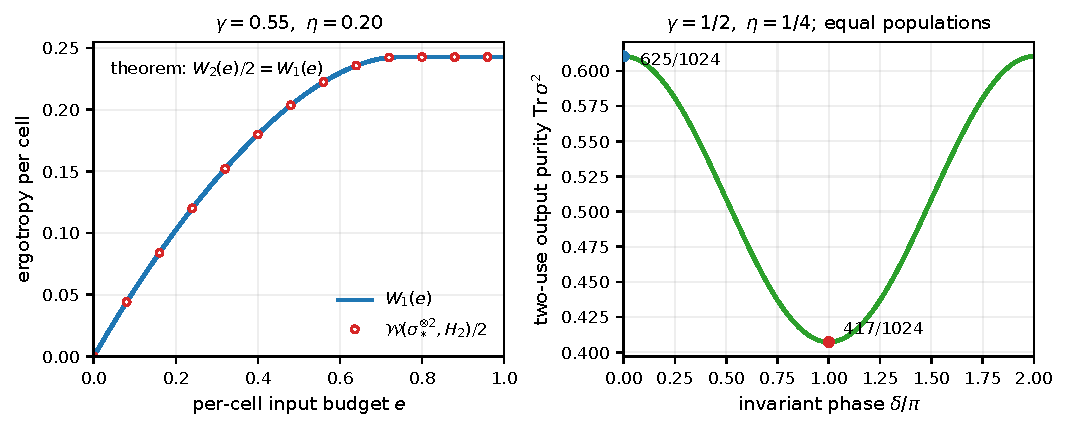
\includegraphics[width=\textwidth]{figures/gadc_two_use_summary.pdf}
\caption{\label{fig:summary}
(a) The one-use optimum from Eq.~\eqref{eq:one-use} (solid curve) and half
the ergotropy of the corresponding two-copy product output, evaluated by a
direct Kraus sum (circles).  The theorem promotes the product value to the
unrestricted two-use optimum $W_2(e)/2$.  The optimizer stops using additional
budget when $e>x_*$.  (b) Output purity for equal input populations as the
invariant phase varies.  The exact values at $\delta=0$ and $\pi$ show why a
real-amplitude or phase-independent reduction cannot certify the theorem.
The plotted data and generation script accompany the manuscript.  OpenAI
Codex (gpt-5.6-sol, Ultra reasoning setting) assisted with the plotting code
and figure generation; deterministic replay reproduced both CSV files
byte-for-byte and the 180-dpi figure raster pixel-for-pixel.}
\end{figure*}

\section{Verification, implications, and limitations}
\label{sec:discussion}

The identities in Eqs.~\eqref{eq:E2}, \eqref{eq:E4},
\eqref{eq:D0-compression}, and \eqref{eq:multiplier} were expanded and reduced
to zero in exact symbolic arithmetic.  Independently transcribed channel
implementations---one summing the sixteen product Kraus operators and one
tensoring the Liouville action of Eq.~\eqref{eq:channel-action} with an
explicit index permutation---agree on the full two-qubit operator basis.
They reproduce the one-use formula and product-code equality.  Floating-point
searches over complex pure and mixed inputs provide diagnostics but are not
used as evidence for the universal inequality; the theorem rests on the exact
sign certificate above.  The substantive AI assistance used in the research
and verification workflow is identified in the Acknowledgments; all
machine-produced algebra entering the result was subjected to the exact and
independent checks just described.

Operationally, Eq.~\eqref{eq:theorem} says that an entangling two-cell
encoding cannot improve maximal output ergotropy at a fixed per-cell input
budget under identical, independent GADC noise.  It does not say that every
optimal input is separable, nor does it price the preparation of an entangled
state.  More importantly, the proof is specific to two uses: neither the
four-level spectral identity nor the coefficient reduction establishes the
arbitrary-$n$ conjecture in Ref.~\cite{tirone2025}.  The conclusion also does
not cover interacting cells, correlated noise, ancillas, local-only
extraction, feedback, postselection, or intermediate control.

\section*{Data availability}

The exact symbolic checkers, the independent Kraus and Liouville channel
implementations, captured verification logs, and the source data and script
for Fig.~\ref{fig:summary} accompany this local manuscript package.  No
experimental data were used.  A permanent public repository identifier must
be chosen by the author before submission.

\begin{acknowledgments}
OpenAI Codex using the gpt-5.6-sol model with the Ultra reasoning setting was
used substantively for scientific reasoning, symbolic-code development,
independent computational checks, literature organization, and manuscript
drafting.  The research scope and quantified claim were explicitly frozen by
the author.  AI-produced algebra was checked by exact symbolic identities,
independent Kraus/Liouville implementations, and a separate AI referee replay.
This local draft still requires complete human scientific and textual review;
before any submission the author must review and refine the work and assume
full responsibility for its accuracy.
\end{acknowledgments}

\appendix

\section{Full phase-dependent output and the reference determinant}
\label{app:output}

For the state in Eq.~\eqref{eq:pure-state}, the diagonal entries of
$\sigma=\Phi_{\gamma,\eta}^{\otimes2}(|\psi\rangle\langle\psi|)$ in the
ordered basis $(|00\rangle,|01\rangle,|10\rangle,|11\rangle)$ are
\begin{align}
z_0&=(1-u)^2A+(1-u)dS+d^2P,\nonumber\\
z_1&=u(1-u)A+(1-u)(1-d)B+udC+d(1-d)P,\nonumber\\
z_2&=u(1-u)A+udB+(1-u)(1-d)C+d(1-d)P,\nonumber\\
z_3&=u^2A+u(1-d)S+(1-d)^2P.
\label{eq:zentries}
\end{align}
Its upper-triangular off-diagonal entries are
\begin{align}
\sigma_{01}&=\sqrt q\bigl[(1-u)\sqrt{AB}+d\sqrt{CP}e^{-i\delta}\bigr],\nonumber\\
\sigma_{02}&=\sqrt q\bigl[(1-u)\sqrt{AC}+d\sqrt{BP}e^{-i\delta}\bigr],\nonumber\\
\sigma_{03}&=q\sqrt{AP}e^{-i\delta},\qquad \sigma_{12}=q\sqrt{BC},\nonumber\\
\sigma_{13}&=\sqrt q\bigl[u\sqrt{AC}+(1-d)\sqrt{BP}e^{-i\delta}\bigr],\nonumber\\
\sigma_{23}&=\sqrt q\bigl[u\sqrt{AB}+(1-d)\sqrt{CP}e^{-i\delta}\bigr].
\label{eq:offdiag}
\end{align}
The lower-triangular entries are fixed by Hermiticity.

To specify $D_0$ in Eq.~\eqref{eq:E4}, choose $B=S$, $C=0$ and define
\begin{align}
z_1^{(0)}&=u(1-u)A+(1-u)(1-d)S+d(1-d)P,\nonumber\\
z_2^{(0)}&=u(1-u)A+udS+d(1-d)P,
\end{align}
and
\begin{gather}
a_{01}=\sqrt{qAS}(1-u),\quad a_{02}=\sqrt{qSP}\,d,
\quad a_{03}=q\sqrt{AP},\nonumber\\
a_{13}=\sqrt{qSP}(1-d),\qquad a_{23}=\sqrt{qAS}\,u.
\end{gather}
Then the explicitly polynomial expression (each displayed square-root product
has integer powers) is
\begin{align}
D_0={}&z_0z_1^{(0)}z_2^{(0)}z_3-a_{01}^2z_2^{(0)}z_3
-a_{02}^2z_1^{(0)}z_3\nonumber\\
&-a_{03}^2z_1^{(0)}z_2^{(0)}-a_{13}^2z_0z_2^{(0)}
-a_{23}^2z_0z_1^{(0)}\nonumber\\
&+a_{01}^2a_{23}^2+a_{02}^2a_{13}^2\nonumber\\
&-2a_{01}a_{02}a_{13}a_{23}
+2a_{01}a_{03}a_{13}z_2^{(0)}\nonumber\\
+2a_{02}a_{03}a_{23}z_1^{(0)}.
\label{eq:D0}
\end{align}
Expanding Eqs.~\eqref{eq:zentries}--\eqref{eq:offdiag} gives
Eqs.~\eqref{eq:E2} and \eqref{eq:E4}; no phase-independent ansatz is used.

\section{Exact-check map}
\label{app:checks}

The accompanying checker first constructs the entries in
Eqs.~\eqref{eq:zentries}--\eqref{eq:offdiag} with a Laurent variable for
$e^{i\delta}$ and verifies Eq.~\eqref{eq:E4} by exact fraction-free
elimination.  A second checker expands the following identities independently:
\begin{enumerate}
\item $X=qK+J$ and $KD_0-4APudX^2=SRJ^2$;
\item the multiplier identity \eqref{eq:multiplier};
\item $F-2q\tau=g^2$ and the nonnegative remainder \eqref{eq:R0};
\item the interval identity \eqref{eq:H-bound}, the one-use identity
\eqref{eq:r-de}, and the spectral identity \eqref{eq:spectral-sos}.
\end{enumerate}
All of these checks are exact polynomial reductions.  The numerical routines
then compare the two channel representations and evaluate boundary-realizing
states; they are retained to catch transcription and basis-order errors, not
to replace the proof.

\bibliography{references}

\end{document}
